\begin{figure}
    \centering
    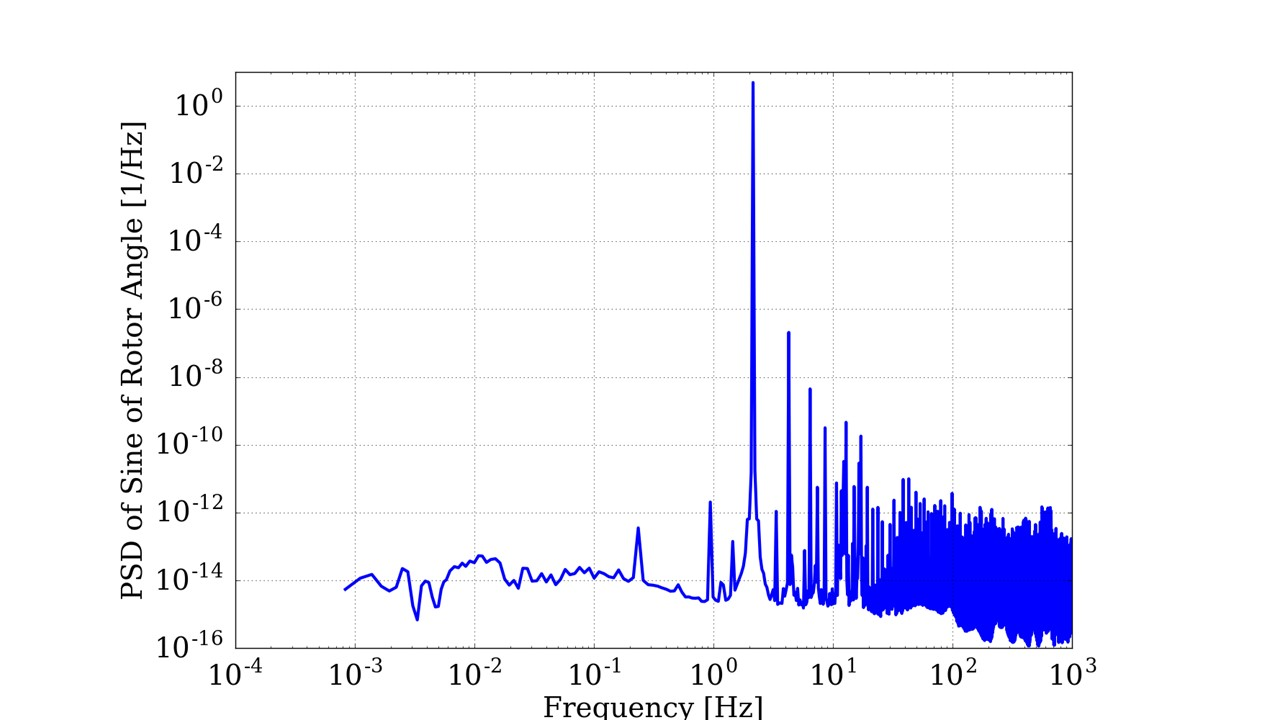
\includegraphics[width=0.98\linewidth]{CHWPEvaluation/Figures/chwp_sine_angle.jpg}
    \caption[CHWP modulation function power spectral density]{Power spectral density of the CHWP modulation function, as measured in a standalone test setup of the CHWP rotator. The white noise level is $\sim$ 0.1 $\mu$ s, which is well within the timing resolution needed to suppress noise associated with CHWP angle jitter below the expected noise level of the inverse-variance-weighted noise-equivalent power for the detector array.}
    \label{fig:chwp_mod_func_psd}
\end{figure}

\begin{figure}
    \centering
    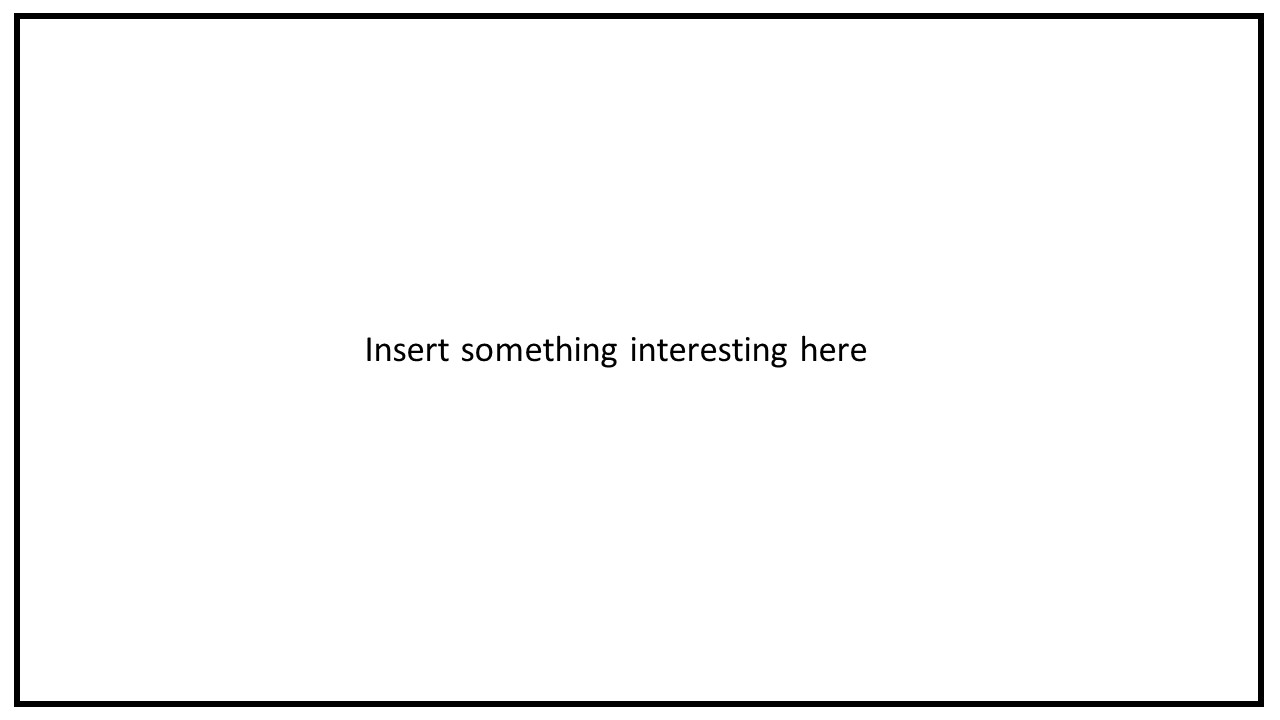
\includegraphics[width=0.98\linewidth]{Other/empty.jpg}
    \caption[Beaglebone IRIG power spectral density]{Power spectrum of the IRIG-B riming signal, which is broadcasted once every second. The white noise level represent es the sampling noise introduced by the Beaglebone, and this measurement demonstrates that this noise level is below that expected from other sources in the CHWP DAQ.}
    \label{fig:chwp_bbb_irig_psd}
\end{figure}

\begin{figure}
    \centering
    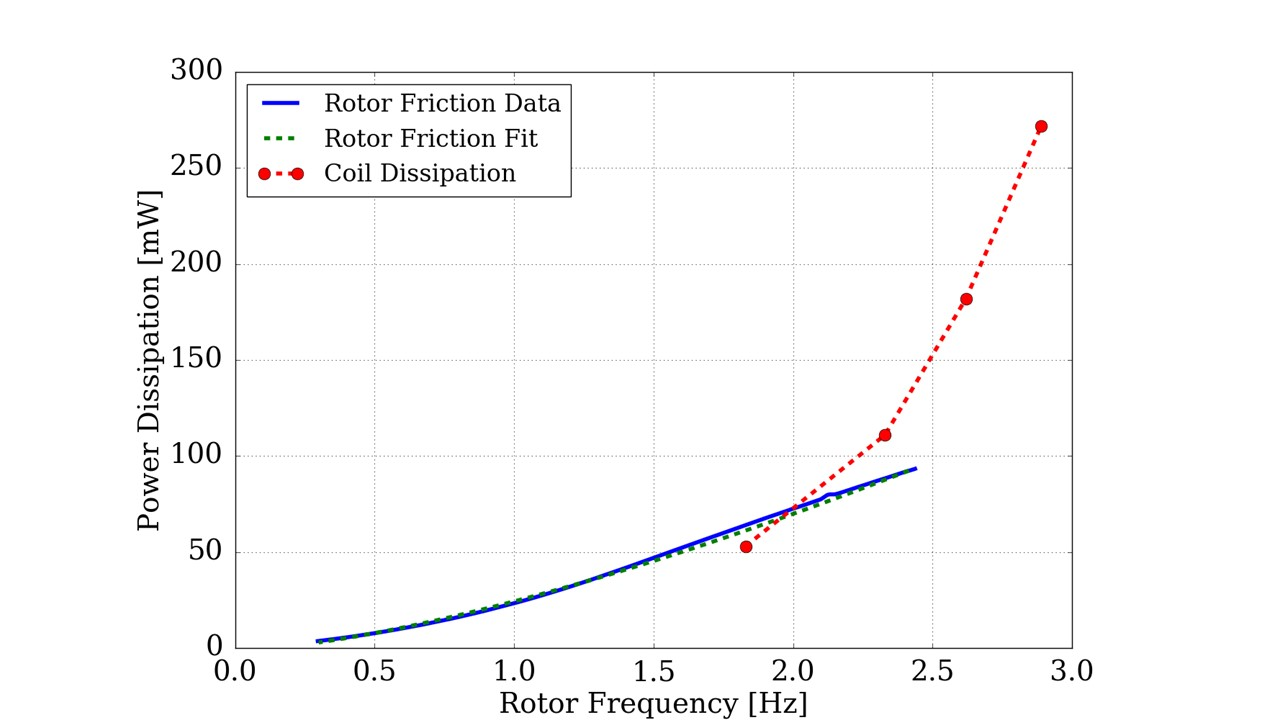
\includegraphics[width=0.98\linewidth]{CHWPEvaluation/Figures/chwp_power_dissipation.jpg}
    \caption[CHWP cryogenic power dissipation]{Measured CHWP cryogenic power dissipation vs CHWP rotation frequency. The blue line represents power dissipated by the rotor due to friction and is estimated by measuring the deceleration of the rotor vs frequency with the motor power off. The red line represents the power dissipated in the drive coils, measured by probing both the voltage over the coils and the series resistance of the coils. The exponential trend is associated with the fact that the motor becomes less efficient at higher frequencies due to the inductive phase shift.}
    \label{fig:chwp_power_dissipation}
\end{figure}

\begin{figure}
    \centering
    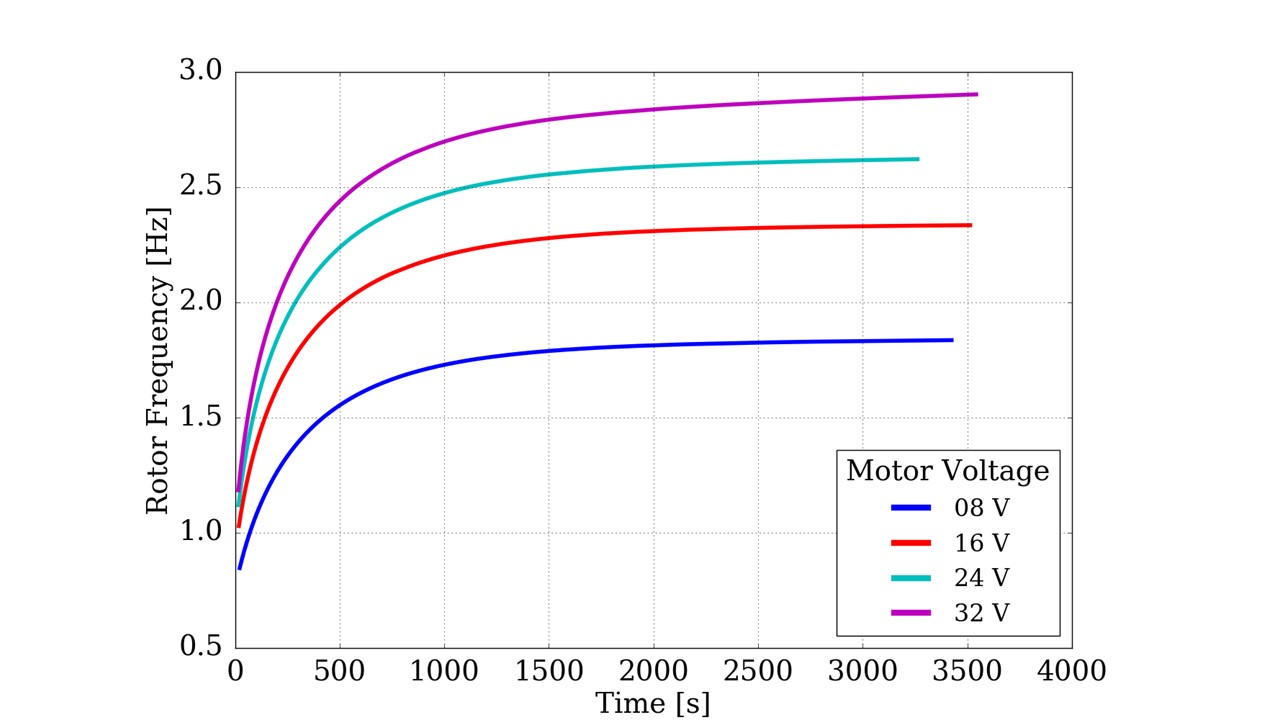
\includegraphics[width=0.98\linewidth]{CHWPEvaluation/Figures/chwp_startup_curves.jpg}
    \caption[CHWP rotation frequency vs time when starting for various motor voltages]{CHWP rotation frequency vs time when starting for various motor voltages. This test demonstrates that the rotor spins to full speed in a reasonable amount of time, and conversely, that it can be stopped in a reasonable amount of time, which is important for rotor recovery in the event of a power outage. TODO: ADD SPINDOWN CURVES}
    \label{fig:chwp_spinup_curves}
\end{figure}